\documentclass[]{book}
\usepackage{lmodern}
\usepackage{amssymb,amsmath}
\usepackage{ifxetex,ifluatex}
\usepackage{fixltx2e} % provides \textsubscript
\ifnum 0\ifxetex 1\fi\ifluatex 1\fi=0 % if pdftex
  \usepackage[T1]{fontenc}
  \usepackage[utf8]{inputenc}
\else % if luatex or xelatex
  \ifxetex
    \usepackage{mathspec}
  \else
    \usepackage{fontspec}
  \fi
  \defaultfontfeatures{Ligatures=TeX,Scale=MatchLowercase}
\fi
% use upquote if available, for straight quotes in verbatim environments
\IfFileExists{upquote.sty}{\usepackage{upquote}}{}
% use microtype if available
\IfFileExists{microtype.sty}{%
\usepackage{microtype}
\UseMicrotypeSet[protrusion]{basicmath} % disable protrusion for tt fonts
}{}
\usepackage[margin=1in]{geometry}
\usepackage{hyperref}
\hypersetup{unicode=true,
            pdftitle={FlipAround},
            pdfauthor={Authored by, and for MDSI students},
            pdfborder={0 0 0},
            breaklinks=true}
\urlstyle{same}  % don't use monospace font for urls
\usepackage{natbib}
\bibliographystyle{plainnat}
\usepackage{longtable,booktabs}
\usepackage{graphicx,grffile}
\makeatletter
\def\maxwidth{\ifdim\Gin@nat@width>\linewidth\linewidth\else\Gin@nat@width\fi}
\def\maxheight{\ifdim\Gin@nat@height>\textheight\textheight\else\Gin@nat@height\fi}
\makeatother
% Scale images if necessary, so that they will not overflow the page
% margins by default, and it is still possible to overwrite the defaults
% using explicit options in \includegraphics[width, height, ...]{}
\setkeys{Gin}{width=\maxwidth,height=\maxheight,keepaspectratio}
\IfFileExists{parskip.sty}{%
\usepackage{parskip}
}{% else
\setlength{\parindent}{0pt}
\setlength{\parskip}{6pt plus 2pt minus 1pt}
}
\setlength{\emergencystretch}{3em}  % prevent overfull lines
\providecommand{\tightlist}{%
  \setlength{\itemsep}{0pt}\setlength{\parskip}{0pt}}
\setcounter{secnumdepth}{5}
% Redefines (sub)paragraphs to behave more like sections
\ifx\paragraph\undefined\else
\let\oldparagraph\paragraph
\renewcommand{\paragraph}[1]{\oldparagraph{#1}\mbox{}}
\fi
\ifx\subparagraph\undefined\else
\let\oldsubparagraph\subparagraph
\renewcommand{\subparagraph}[1]{\oldsubparagraph{#1}\mbox{}}
\fi

%%% Use protect on footnotes to avoid problems with footnotes in titles
\let\rmarkdownfootnote\footnote%
\def\footnote{\protect\rmarkdownfootnote}

%%% Change title format to be more compact
\usepackage{titling}

% Create subtitle command for use in maketitle
\newcommand{\subtitle}[1]{
  \posttitle{
    \begin{center}\large#1\end{center}
    }
}

\setlength{\droptitle}{-2em}
  \title{FlipAround}
  \pretitle{\vspace{\droptitle}\centering\huge}
  \posttitle{\par}
  \author{Authored by, and for MDSI students}
  \preauthor{\centering\large\emph}
  \postauthor{\par}
  \predate{\centering\large\emph}
  \postdate{\par}
  \date{V:2017-03-06}

\usepackage{booktabs}
\usepackage{amsthm}
\makeatletter
\def\thm@space@setup{%
  \thm@preskip=8pt plus 2pt minus 4pt
  \thm@postskip=\thm@preskip
}
\makeatother

\usepackage{amsthm}
\newtheorem{theorem}{Theorem}[chapter]
\newtheorem{lemma}{Lemma}[chapter]
\theoremstyle{definition}
\newtheorem{definition}{Definition}[chapter]
\newtheorem{corollary}{Corollary}[chapter]
\newtheorem{proposition}{Proposition}[chapter]
\theoremstyle{definition}
\newtheorem{example}{Example}[chapter]
\theoremstyle{remark}
\newtheorem*{remark}{Remark}
\begin{document}
\maketitle

{
\setcounter{tocdepth}{1}
\tableofcontents
}
\chapter{Welcome}\label{welcome}

The purpose of this document is to ensure that all MDSI students have a
source that will help to `wing' the ride that is MDSI, to ensure that
something exists to help the hectic ride that is Data Science and
provides easy resources and easy links to information that can help you.

\section{Welcome message}\label{welcome-message}

MDSI is unique in its approach and feel. MDSI is a `boutique degree'
which means we are a small tight-knit data family which means the
contacts you walk out (really) knowing are going to be more valuable
than the skills you learn. In terms of content, our point of difference
is the innovation in our name. We take our innovation component as
seriously as data science, and is ingrained in everything that's taught.
For us, a data science degree was our innovation (we were the first of
its kind in Australia), and in the rapidly changing context that is
data, the ability to innovate and adapt is a pretty great point of
difference for you too.

Data science is a collaborative discipline. Students in the MDSI program
get hands on experience of working in teams to formulate and solve
real-life data science problems. Most courses focus on techniques to
solve problems, but spend very little time (if any) on how problems
should be formulated. The MDSI program is structured in a way that helps
students learn this tacit, but crucial skill.

Another important aspect of data science is that it is a rapidly
evolving field. A data scientist must therefore be able to stay current
with developments in the field. The MDSI program, with its emphasis on
critical self-learning, prepares students to be lifelong learners.

Welcome, and good luck on your MDSI journey

\section{Checklist of things to do}\label{checklist-of-things-to-do}

Getting started on your MDSI journey can be somewhat overwhelming. So to
help you ease into life as an MDSI student, the following checklist will
help you to get up and running as painlessly as possible.

\begin{itemize}
\tightlist
\item
  Do your statistics pre-flight test
\item
  Activate UTS student email
\item
  Forward UTS student email if required
\item
  Enrol in your subjects
\item
  Review Subject Outlines
\item
  Activate and personalise CICAround
\item
  Join the Slack Channel
\item
  Do your CLARA profile
\item
  Download R \& R Studio
\item
  Download Tableau
\item
  Activate Github
\item
  Download Python \& Rodeo (optional)
\item
  Download Rapidminer (optional)
\item
  Test your Google Drive
\item
  Test your Office 365 Drive
\item
  Download Quantum GIS (optional)
\item
  Download KNIME (optional)
\item
  Log into Diigo
\item
  Log into SPARK
\item
  Log into Review
\end{itemize}

\section{Pre-flight tests}\label{pre-flight-tests}

MDSI statistics pre-flight test:
\url{http://www.uts.edu.au/future-students/analytics-and-data-science/essential-information/mdsi-statistics-pre-flight-test}

\section{MDSI Jargon}\label{mdsi-jargon}

\begin{tabular}{l|l}
\hline
Jargon & Description\\
\hline
UTS Online & UTS’s Online learning system\\
\hline
CICAround & CIC’s blog environment where students can post blogs about their studies and learning\\
\hline
FlipAround & A student guide developed by students for students in a collaborative environment\\
\hline
CIC Squared & Social networking event where students, staff and industry can connect\\
\hline
R & A coding language used in data science\\
\hline
Python & A coding language used in data science\\
\hline
KNIME & A algorithm building tool\\
\hline
Diigo & A collection of resources contributed by the MDSI community\\
\hline
Slack & A ‘chat’ type application completely driven by the student community.\\
\hline
WordPress & The host of CICAround\\
\hline
Lynda.com & An online learning platform with many free courses\\
\hline
MOOC & Massive Open Online Course\\
\hline
Hackathon & An event, typically lasting several days, where people collaborate to find information in data\\
\hline
Azure & Microsoft’s cloud computing platform\\
\hline
AWS & Amazon Web Services’ cloud computing services\\
\hline
Coursera & Website host/ service provider of MOOC’s\\
\hline
GA & Graduate Attribute\\
\hline
CILO & Course Intended Learning Outcome\\
\hline
SLO & Subject Learning Outcome\\
\hline
\end{tabular}

\chapter{The data science mindset}\label{the-data-science-mindset}

\section{CLARA}\label{clara}

Each person has their own learning preferences and habits of mind that
shape their response to challenges and learning opportunities.

CLARA (Crick LeArning for Resilient Agency) is a tool used to prompt
reflection on a multidimensional construct called ``Learning Power''
with eight dimensions: curiosity, creativity, sense making, belonging,
collaboration, hope and optimism, mindful agency and openness to change.
The UTS Graduate Attributes have a strong resonance with these
dimensions. The CLARA tool is used as part of MDSI activities, aiming to
help the students maximise their development results through
understanding themselves better, namely with regards to their approach
to learning and challenges.

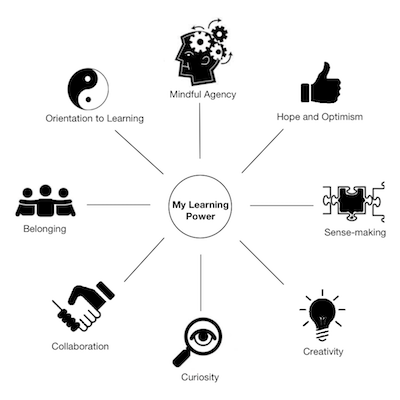
\includegraphics{Images/CLARAspider.png}

The tool is survey-based and provides a profile-style feedback covering
each of the following dimensions:

Curiosity

\begin{itemize}
\tightlist
\item
  Wanting to get beneath the surface \& find out more
\item
  Always wondering why and how
\end{itemize}

Creativity

\begin{itemize}
\tightlist
\item
  Using my intuition \& imagination to generate new ideas \& knowledge
\item
  Taking risks \& playing with ideas and artefacts to arrive at new
  solutions
\end{itemize}

Sense making

\begin{itemize}
\tightlist
\item
  Making connections between what I already know \& new information \&
  experience
\item
  Making meaning by linking my story, my new learning \& my purpose
\end{itemize}

Belonging

\begin{itemize}
\tightlist
\item
  Being part of a learning community at work, at home, in education \&
  in my social networks
\item
  Knowing I have social resources to draw on when I need them
\end{itemize}

Collaboration

\begin{itemize}
\tightlist
\item
  Being able to work with others, to collaborate and co-generate new
  ideas and artefacts
\item
  Being able to listen and contribute productively to a team
\end{itemize}

Hope and optimism

\begin{itemize}
\tightlist
\item
  Having the optimism \& hope that I can learn \& achieve over time
\item
  Having a growth mindset; believing I can generate my own new knowledge
  for what I need to achieve Mindful agency
\item
  Taking responsibility for my own learning over time through defining
  my purposes, understanding and managing my feelings,
\item
  Knowing how I go about learning \& planning my learning journey
  carefully Openness to change
\item
  An emotional orientation of being open \& ready to invest in learning,
  having flexible self-belief, willing to persist \& manage any
  self-doubt
\item
  A necessary prerequisite for developing resilience in learning
\end{itemize}

Here is an example of an output from CLARA, showing the resulting
profile, based on the responses provided in the survey.

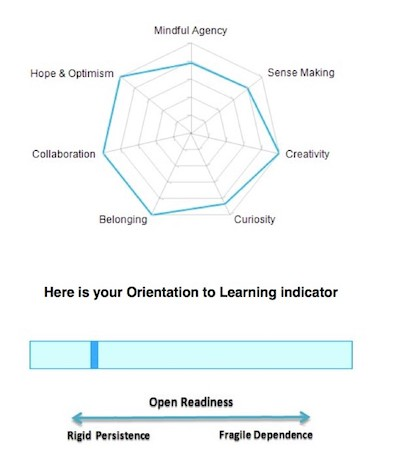
\includegraphics[width=0.5\linewidth]{Images/Clara}

Learning profiles can change over time, so MDSI conducts two sets of
CLARA tests, to allow the students to compare their profile changes and
reflect on their development progress.

CLARA survey will be organised by MDSI and each student will receive a
link and instructions on how to utilise this tool.

\section{Data Science Professional
Competencies}\label{data-science-professional-competencies}

Competency can be defined as ``effective application of skill, knowledge
and abilities to on-the-job-behaviour and capability to perform to job
requirements''. MDSI supports the ongoing development professional
development efforts and offers a tool that can help the students
evaluate their skills and abilities in various domains associated with
the data science professional competencies. Students are encouraged to
utilise the tool to identify the key competencies associated with their
individual career aspirations. For each relevant competency, students
evaluate their current competency levels, identify any gaps and use the
information to create a set of actions that would form their
professional development plan. The competencies model is introduced to
students as part of 36100 (Data Science and Innovation) subject through
a self-assessment exercise. The competencies are divided into two
groups: technical and managerial, describing the following competency
(proficiency) levels for each domain: Beginner, Competent, Advanced and
Expert.

\textbf{Technical:}

\begin{itemize}
\tightlist
\item
  Mathematics and statistics
\item
  Programing and scripting languages
\item
  Databases and data storage
\item
  Computing systems, platforms, security, integration
\item
  Data mining
\item
  Data modelling
\item
  Analytics, predictive modelling and machine learning
\item
  Data visualisation
\item
  Business analysis and interpretation
\item
  Product development
\end{itemize}

\textbf{Interpersonal/managerial:}

\begin{itemize}
\tightlist
\item
  Creativity
\item
  Communication
\item
  Data strategy
\item
  Line management
\item
  Data management and governance
\item
  Facilitation and presentation
\item
  Project management
\end{itemize}

\textbf{Competency levels:}

\begin{itemize}
\tightlist
\item
  \textbf{Beginner:} able to assist and perform simple tasks
\item
  \textbf{Competent:} able to perform tasks independently
\item
  \textbf{Advanced:} able to perform complex tasks
\item
  \textbf{Expert:} able to perform complex transformative, strategic or
  trans-disciplinary tasks
\end{itemize}

The competencies assessment exercise aims to prompt the students to take
a proactive attitude to their professional development efforts and
effectively apply their analytical skills, dedication and
professionalism in managing their career objectives.

The competencies assessment exercise covers the following steps:

\begin{enumerate}
\def\labelenumi{\arabic{enumi}.}
\tightlist
\item
  Evaluate your current competency level for each domain on the list
\item
  Choose a set of domains (no more than 6) that are relevant to your
  planned development for this subject, your course and your career
  goals.
\item
  Identify the goal competency levels for the selected domains and
  describe related professional development outcomes that support your
  assessment
\item
  Analyse your development outcomes in the context of your career goals
  and identify the gaps between your current and goal competency levels
\item
  Develop a set of actions needed to achieve desired level of
  competencies and bridge the identified gap
\item
  Provide feedback and suggestions for the improvement of the current
  list of competencies, descriptions etc.
\end{enumerate}

\section{Ethics amd Privacy}\label{ethics-amd-privacy}

Its important to understand that security, privacy and ethics are three
different things, although heavily intertwined in the `internet of
things'.

What is ethical when it comes to data and the internet of things? Is
privacy having a login or not being identifiable as an individual?

The world of Ethics and Privacy is changing, similar to the definition
that now includes much more than it did a decade ago. Computer security
like a login is no longer sufficient to providing protection of privacy
which is more focused on ensuring that only people who should have the
authority to access your information should be able to.

Current Privacy legislation addresses control and authentication
processes of whom can access your information via direct disclosures and
how this information should be stored by the party who is collecting
this information, it does not address disclosures that can be made based
on inferences that can be drawn from big data of which your information
is a part. Is the value or conclusions that could be drawn from
information as part of big data considered private information?

A sensible framework in relation to Ethics and Privacy where data is
concerned is highlighted in the Belmont report which identifies two
rules to consider ``(1) do not harm and (2) maximize possible benefits
and minimize possible harms.''

A big ethical dilema of late is the rich data sources that various
provider hold, that if pooled together will strip all possibility of
anonymity.

For more on this read:

\url{http://www.tandfonline.com/doi/full/10.1080/08900523.2014.863126?src=recsys}
\url{http://libres.uncg.edu/ir/uncg/f/N_Kshetri_Big_2014.pdf}

\section{Digital Footprint}\label{digital-footprint}

Your digital footprint
\url{https://en.wikipedia.org/wiki/Digital_footprint} is the name given
to the data that is recorded about you all day every day. It can be the
time and phone number of someone that you called, the mobile phone tower
that you were connected to at the time of making the call and how long
you spoke for. It is the IP address of your computer when you connect to
the internet. It is the list of items you pay for when you go through
the checkout at the supermarket and the eftpos card number you used to
pay for the items. It is the surveillance footage you appear in when you
move through monitored public spaces. It is stories you `like' or share
on social media sites. It is the journeys that your GPS navigation
stores about your travels. It is every email you send and every click
you make when you browse the internet.

Your digital footprint is the inescapable record of your existence by
doing nothing more than living your life. It is an important aspect of
modern society as many services that you enjoy depend on the data you
generate in order to provide critical services. A bank can't tell you
how much money you have without keeping record of your bank
transactions. For good or for evil, this data comes embedded with far
more information about you. By looking at the kinds of things you spend
your money on or the businesses that you spend your money at and the
time of day that you spend your money there, it can be determined where
you live and where you work.

As an MDSI student, you will learn to think critically and ethically
about data collection and how it can be used for good and for evil. The
best place to start your thinking is with your own digital footprint,
become aware of how big it is and how you feel about it.

It's important to note that very little permission is sought on data
collection and when it is sought, very little education is provided in
terms of the use of that data. Very few providers who collect data
clarify or specify what the data they collect is used for.

You are responsible for your digital footprint. Generate it wisely.

\section{Opportunity for overseas
exchange}\label{opportunity-for-overseas-exchange}

Some great opportunities exist within MDSI with our Program Director
having many contacts in many other countries which enable us to be able
to explore greater opportunities for overseas exchange.

You need to do a few things before this opportunity is explored as set
out by the Program Director to ensure for an easier way forward if this
is an opportunity you want to explore.

\section{Electives}\label{electives}

You need to select four electives during your MDSI course. These
electives should be selected to assist you in your growth as a student
and as a data science professional. These subjects enable you to add to
your toolbox of where you are heading with your journey.

Electives can be selected from any school however you will still be
subjected to the pre-requisites for any possible subject, so it will
depend on the requirements of the subject.

We suggest that when you apply for a subject with a prerequisite that
you also apply for a waive of the prerequisite if the prerequisite is a
subject you are familiar with but have not done with UTS and get
exemption for that requisite.

This is not always easy, or approved and is subject to each School's
internal views or policies. It is definitely a consideration to take.

You can apply for the subject ( and a waiver of prerequisites if
required) early as CIC is not limited by inter-faculty time
restrictions.

Our best tip is : get in early.

\chapter{\texorpdfstring{A `survival guide' to
MDSI}{A survival guide to MDSI}}\label{a-survival-guide-to-mdsi}

\section{First steps}\label{first-steps}

\subsection{Your UTS email:}\label{your-uts-email}

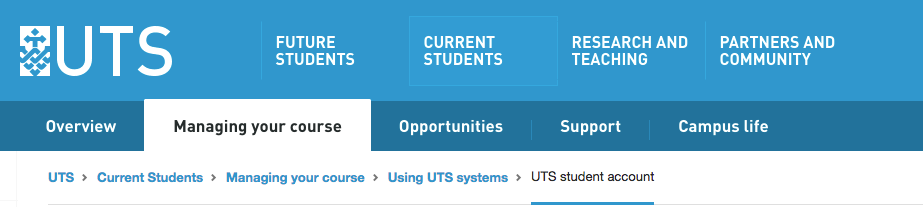
\includegraphics{images/UTSmanagecourseBanner.png}

First and foremost you need to activate your UTS email address. All
official communications from UTS, subject notifications, MDSI
newsletters etc will be sent to this email address. You need to activate
your email address before you can access other UTS systems.

\textbf{Activate your UTS Student email:}

\begin{itemize}
\tightlist
\item
  Navigate to
  \url{https://email.itd.uts.edu.au/webapps/myaccount/activation/} and
  follow the steps to activate your UTS student email account.
\item
  ** Protip: ** If you don't want to login frequently to check if you
  have mail, simply setup a email forwarding to an email address of your
  choice via the settings page after logging in.
\end{itemize}

For more general information about using UTS systems go to:
\url{http://www.uts.edu.au/current-students/managing-your-course/using-uts-systems/uts-student-account}

\subsection{Enrol in your subjects:}\label{enrol-in-your-subjects}


\includegraphics{Images/StudentAdmin.png}

It is really important that you check your enrolment. If you are not
enrolled, you cannot participate in your studies. This might seem
obvious, however at UTS you need to do more than simply accept your
offer. Once you have received and accepted your offer to study, you then
need to enrol into your subjects.

If you have not enrolled, you need to login into the My Student Admin
\url{https://onestopadmin.uts.edu.au/estudent/Login.aspx} portal to
enrol.

For more information about enrollment and a step by step instruction
guide, please visit:

\url{http://www.uts.edu.au/current-students/managing-your-course/your-enrolment/how-enrol}

\subsection{Get your subject outlines:}\label{get-your-subject-outlines}

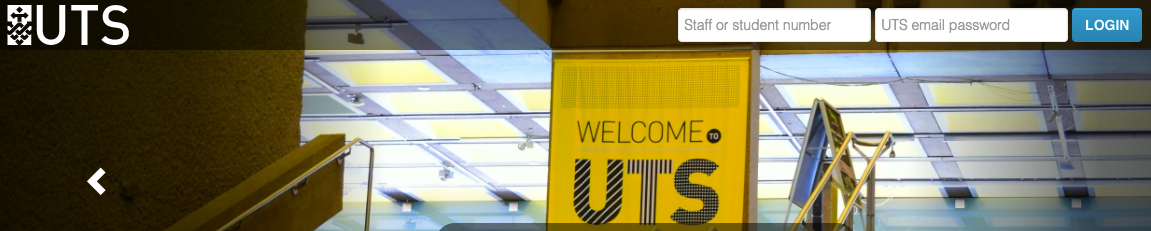
\includegraphics{images/UTSOnline.png} MDSI uses a variety of systems
for online teaching and learning. UTSOnline
\url{https://online.uts.edu.au/} and CICAround
\url{https://ca.uts.edu.au} are the two primary environments for you to
familiarise yourself with.

The first thing you need to do after activating your email address is to
login to UTSOnline, access your subjects and find your subject outline.
Your subject outline contains everything you need to know about your
subject for the coming semester. It includes the contact information for
your subject co-ordinator, important dates, assessment descriptions and
much more. In most cases you can find the answer to any question you
might have about your subject addressed in the subject outline.

\textbf{Find your subject outlines in UTSOnline:}

\begin{itemize}
\tightlist
\item
  Login to UTSOnline at \url{https://online.uts.edu.au/} using your
  student ID number and the password you setup for your UTS email
  account.
\item
  Access your subjects by clicking on your subject name
\item
  Download your subject outline by clicking on the link titled `Subject
  Outline' in the left side menu, then click on the subject outline link
  on the page.
\end{itemize}

\subsection{Join the MDSI community:}\label{join-the-mdsi-community}


\includegraphics{images/CAlogo.png}

Your next stop should be CICAround. Here you will connect with your
peers in an academic capacity. There are discussion forums for your
subjects where you can post questions. CICAround most notably is where
you will go to blog about your experiences throughout your MDSI journey.
The first step is to activate your blog. Then you can browse through the
blogs of your new MDSI family and read about their experiences and the
things they have learnt.

\textbf{Activate and personalise your CICAround profile:}

\begin{itemize}
\tightlist
\item
  Navigate to \url{https://ca.uts.edu.au/using-ca/}
\item
  Watch the welcome video then login to CICAround using your student ID
  and password.
\item
  Put up your first CICAround Blog post
\end{itemize}

\subsection{Join the MDSI chatter:}\label{join-the-mdsi-chatter}


\includegraphics{images/Slacklogo.png}

Slack has proven to be a very useful tool so far. It is completely
driven by the student community and is where the MDSI student community
goes to socialise, organise BBQs, ask each other for technical help and
share useful resources. If you need a quick answer, Slack is the place
to go.

\textbf{Join the Slack Channel}

\begin{itemize}
\tightlist
\item
  You can download the Slack application from
  \url{https://slack.com/downloads}
\item
  You can also get the app for IOS, Android and Windows phones.
\item
  You do not need to pay for a subscription.
\item
  Sign Up to the MDSI group at: \url{https://utsmdsi.slack.com/}
\end{itemize}

If you're completely new to Slack, there are some helpful getting
started guides at
\url{https://get.slack.help/hc/en-us/categories/202622877-Slack-Guides}

\section{Technology}\label{technology}

\subsection{R / R Studio}\label{r-r-studio}


\includegraphics{Images/RStudiologo.png}

`R' is a coding language used by most of the data science community.
RStudio is a software program or `Integrated Development Environment'
(IDE) that makes working with the R language ALOT easier. The
programming environment is really flexible as it allows you the joy of
working in a notebook format, scripting, markdown and publishing your
work as a PDF.

You will use R in many of your subjects and being able to use it well
will give you a serious edge over your classmates and competitors at
hackathons.

\textbf{Download and install R \& RStudio free}

\begin{itemize}
\tightlist
\item
  Download and install the R language: \url{https://cran.rstudio.com/}
\item
  Download and install RStudio IDE:
  \url{https://www.rstudio.com/products/rstudio/download/}
\end{itemize}

\textbf{Libraries well worth their weight in gold:}

\begin{itemize}
\tightlist
\item
  tidyverse \url{http://tidyverse.org/} A collection of libraries that
  make data analysis easier

  \begin{itemize}
  \tightlist
  \item
    readr \url{http://readr.tidyverse.org/} for reading all kinds of
    data formats
  \item
    stringr \url{http://stringr.tidyverse.org/} for working with text
  \item
    ggplot2 \url{http://ggplot2.tidyverse.org/} for visualising data
  \item
    tidyr \url{http://tidyr.tidyverse.org/} for creating tidy data
  \item
    dplyr \url{https://github.com/hadley/dplyr} for manipulating data
  \end{itemize}
\item
  caret \url{http://topepo.github.io/caret/index.html} for creating
  predictive models
\item
  Bookdown \url{https://bookdown.org/} for creating beautiful documents
\end{itemize}

There are many resources to get you started in doing data science with
R. Refer to the resources section for more information.

\subsection{Tableau}\label{tableau}


\includegraphics[width=0.3\linewidth]{images/Tableaulogo}

Tableau is a tool for visualising data. It is quite powerful in its
ability to connect to a variety of data sources both on your computer
and through the internet. It is also relatively intuitive to use.

As a student you can apply to the company for a free license to their
commercial desktop version.
\url{https://www.tableau.com/academic/students}

\subsection{Github}\label{github}


\includegraphics[width=0.3\linewidth]{images/GithubEdulogo}

Github is a fantastic tool to become familiar with. It is a great place
to store code, collaborate with others and even host your own website or
blog.

Github has a really generous collection of free stuff for students. To
claim yours head over to: \url{https://education.github.com/pack}

\subsection{Python / Rodeo / Jupyter
Notebook}\label{python-rodeo-jupyter-notebook}


\includegraphics{images/Pythonlogo.png}

\includegraphics{images/Anacondalogo.png}

Python is a general purpose coding language widely used by the data
science community. A great place to start is with Anaconda from
Continuum Analytics : \url{https://www.continuum.io/downloads}

Anaconda comes with a `container' management environment called `conda'
and ships with a collection of scientific python libraries that have
optimised for fast computation. It is also really helpful to manage your
libraries and will let you know if there are incompatibilities between
the libraries you are using. This is just the tip of the Anaconda
iceberg.


\includegraphics[width=0.2\linewidth]{Images/Jupyterlogo}

Python for data science is commonly used in a notebook format. To this
end Jupyter notebooks will become a familiar friend. Fortunately it is
included as part of Anaconda. For more info, refer to the resources
section.


\includegraphics[width=0.2\linewidth]{Images/Rodeologo}

If you prefer an `R' style IDE, then Rodeo by Yhat is for you.
\url{https://www.yhat.com/products/rodeo}

If you prefer a traditional IDE, you can get a free license for PyCharm
(as well as all their other products) from JetBrains using your student
details: \url{https://www.jetbrains.com/student/}

\textbf{Libraries well worth their weight in gold:}

\begin{itemize}
\tightlist
\item
  Numpy \url{http://www.numpy.org/} for working with numerical arrays
\item
  Scipy \url{https://www.scipy.org/scipylib/index.html} for scientific
  computing with python
\item
  Matplotlib \url{http://matplotlib.org/} for visualising data
\item
  Seaborn \url{http://seaborn.pydata.org/index.html} for statistical
  visualisation
\item
  Pandas \url{http://pandas.pydata.org/} for working with data
\item
  Statsmodels \url{http://www.statsmodels.org/stable/index.html} for
  creating statistical models
\item
  Scikit-Learn \url{http://scikit-learn.org/stable/} for doing machine
  learning with python
\item
  Tensorflow \url{https://www.tensorflow.org/} `deep learning' with
  python
\end{itemize}

Note: Python comes in two different flavours: 2.7 and 3.x. You can start
with either version, but it is worth learning what the subtle
differences are (eventually).

\textbf{A couple of blog posts to help you choose between R and Python:}

\begin{itemize}
\tightlist
\item
  R vs Python for Data Science: The Winner is
  \url{http://www.kdnuggets.com/2015/05/r-vs-python-data-science.html}
\item
  R vs Python for Data Science: Summary of Modern Advances
  \url{https://elitedatascience.com/r-vs-python-for-data-science}
\end{itemize}

\subsection{KNIME}\label{knime}


\includegraphics[width=0.3\linewidth]{images/KNIMElogo}

KNIME Analytics Platform is an open source solution that enables quick,
fast data driven designs for machine learning. Its a visual tool to
learn and use when you need to get the job done quickly (without writing
any code) and need to create algorithms quickly but you don't have the
time to learn the mathematics behind the algorithms. Its friendly and
easy to use to find the hidden `story' in the data.

Go to \url{https://www.knime.org/knime-analytics-platform} to download
KNIME for free.

\subsection{Rapidminer}\label{rapidminer}


\includegraphics[width=0.3\linewidth]{images/Rapidminerlogo}

Rapidminer is another visual tool for doing data analysis, modelling and
machine learning. You can get access to their commercial tools using
your student status from
\url{https://rapidminer.com/educational-program/}

\subsection{Quantum GIS}\label{quantum-gis}


\includegraphics[width=0.2\linewidth]{images/QGISlogo}

QGIS is a really nice open source tool for working with geospatial data.
To get started just head over to
\url{http://www.qgis.org/en/site/index.html}

\subsection{Diigo}\label{diigo}


\includegraphics[width=0.3\linewidth]{images/diigologo}

A collection of resources contributed by the MDSI community.

\textbf{Join the Diigo group} - simply create a Diigo account and
request access. \url{https://groups.diigo.com/group/cic_mdsi}

Frequently used search tags include:

\emph{``DSI, DAM, Data, big\_data, case studies, visualization,
teaching\_tools, statistics, stats-thnkg, privacy, Algorithms,
ethicsVSD, realworldDM, video, Analytics, human-machine, history,
data,mining, Data\_science, cisco, R, IoE, TEDtalks, values, QSProject,
Algorithmic, Accountability, industry, sociotechnical, systems, AI,
podcast, professional\_practice, portfolio, storytelling, bbc, QS,
DMonline, innovation, humanismprofessional, development, open\_data,
speculative\_futures, RealWorld, ted, transdisciplinarity, creativity,
algorithm, sociotechnical, BowkerStar, futuresgender, challenge,
data-sets, accountability, digital\_futures, tools, DM, reading, DVN,
equality, infographic''}

\subsection{Google / Office 365}\label{google-office-365}


\includegraphics{Images/GoogleAppslogo.png}
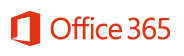
\includegraphics{Images/Office365logo.png}

Your university account allows you access to Google Apps and Office 365.

Google Apps access does not include Gmail. You can not login to your UTS
google apps account via gmail or if you are already logged in with a
personal gmail account, you will need to log out completely from gmail.
Once you have done this, you can log in using your student email
address. This will revert you to a UTS login page. Use your UTS student
number and password and it will revert you back to the Google Drive, but
you will be logged into the drive.

Similarly you can mimic the same steps for Office 365.

\subsection{SPARK-Plus}\label{spark-plus}


\includegraphics[width=0.25\linewidth]{images/SPARKlogo}

SPARK is an acronym for Self and Peer Assessment Review Kit. This tool
has been developed to assist with in class activities as well as being
able to self and peer assess assignments. Its also one of the few tools
that make group assessments/work easier, in particular to marking.

\textbf{Login with your student ID and Password}

\url{https://uts.sparkplus.com.au/login.php}

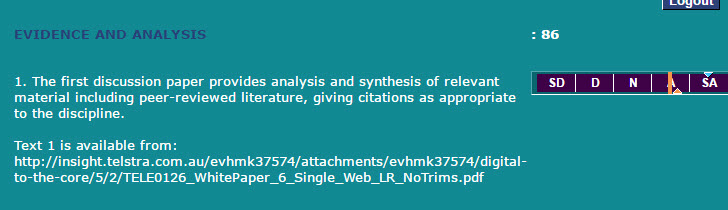
\includegraphics{images/spark.jpg}

\subsection{Review}\label{review}

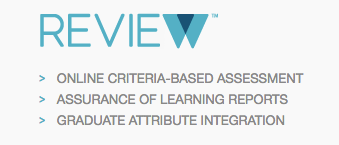
\includegraphics[width=0.4\linewidth]{images/Reviewlogo}

Review is an assessment tool that is used to mark your work, give you
feedback about your work and for you to develop a sense of what is
expected by marking your own work before it is assessed by teaching
staff.

Review allows you to see feedback from your lecturer as well as your
mark broken down by specific GA/CILO set out by your assignment.

It also allows you to self assess your assignment, which allows the
lecturer to see if your expectation is in line with their expectation.
It's important to note that the lecturer will not be able to see your
self assessment until after they have saved your mark.

You are also able to see the average of the class as well as where the
staff has measure you.

\url{https://uts.review-edu.com/uts/}

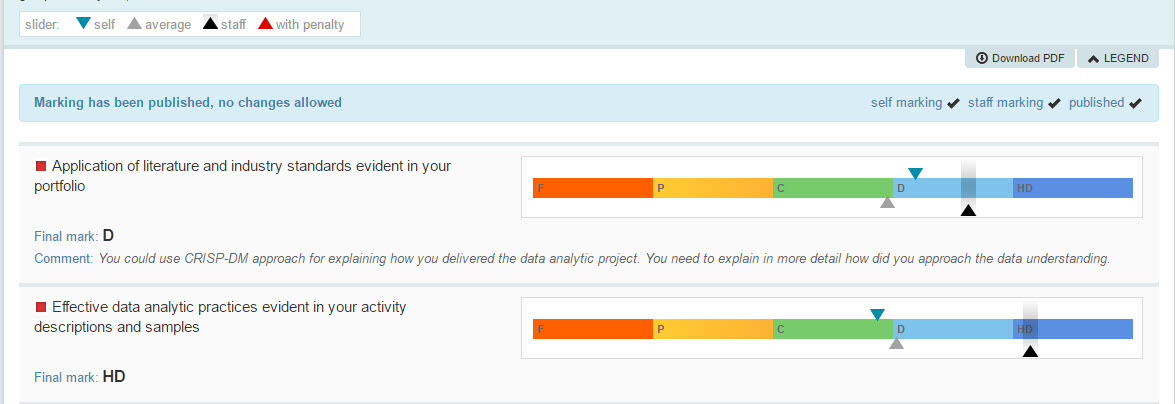
\includegraphics{images/Reviews.jpg}

\section{Writing}\label{writing}

\subsection{Blogs}\label{blogs}

More and more academics and workplaces use blog posts to reach clients,
audiences and share knowledge. Blogs can be useful for many reasons and
is used as a reflective tool for students as well as providing an
opportunity to share any learning.

You can use some tools to turn topics into amazing titles by using
keyword suggesters (\url{http://keywordtool.io}), title generators (
\url{https://www.portent.com/tools/title-maker}), and you can also test
your headlines with the following tool
(\url{http://coschedule.com/headline-analyzer\#})

Tips for new bloggers

\begin{itemize}
\tightlist
\item
  Use an eye catching title
\item
  In-text links
\item
  Use pictures, pictures speak a thousand words
\item
  Keep post to 1000-1500 words
\item
  Use social sharing buttons
\item
  Use paragraphs - one idea per paragraph
\item
  Revise and Rewrite
\item
  Omit needless words - Use the KISS (Keep It Simple, Stupid) Principle
\item
  Use definite, specific concrete language - direct and to the point
\item
  Write in a way that comes naturally - use your active voice
\item
  Be clear - make it simple to read and understand
\item
  Avoid fancy words
\item
  Do not take shortcuts at the cost of clarity
\end{itemize}

Tips on writing blog posts :
\url{https://problogger.com/how-to-write-great-blog-content/} and
\url{http://www.socialmediaexaminer.com/26-tips-for-writing-great-blog-posts/}

\subsection{White papers}\label{white-papers}

Where do you start with a white paper and what are they? White papers
are originally documents written for government policies however this is
most recently being used by companies and universities to get new
policies and research into the public space.

There are some things to consider when writing a white paper:

\begin{itemize}
\tightlist
\item
  Pick a topic people will want to read or a problem you want to solve
\item
  Pick a generic title that describes the problem at hand
\item
  Engage, inform and convince your reader
\item
  Be descriptive and professional
\item
  Consider the audience you are `speaking' to and accommodate for their
  level of expertise
\item
  Set up a great intro
\item
  Emphasize the value you want to or will create
\item
  Decide on a length for the white paper (1-5 pages are the norm)
\item
  Describe the solution you are proposing
\item
  Remember a summary that reviews the problem, solution and result of
  the outcome
\item
  Proofread your document, and ensure someone else reads it before you
  submit/publish it.
\item
  Follow the 3-30-3 rule ( you have three seconds to captures your
  audience's attention from a glance at your piece, if you succeed at
  capturing their attention then you have 30 more seconds to ensure they
  continue reading, if you pass the 3-30 rules then your reader will
  give you three more minutes to make your point).
\end{itemize}

If you would like to enhance your academic writing skills, you might be
interested in have a look at the Academic Phrase Bank:
\url{http://www.phrasebank.manchester.ac.uk/}

\subsection{Assessments}\label{assessments}

The majority of your information regarding a subject and the assessments
is contained in your subject outline. This is your base document and you
should follow it closely. In addition you will get an assignment brief
for each assignment you have due. Its is recommended that you review
these briefs and that you follow the detailed instructions set out for
you.

\section{Research \& Library Access}\label{research-library-access}

Research is something you will do a lot throughout your studies. There
are many contexts that will shape the way you research. For the purposes
of finding academic peer reviewed sources, some tips below will likely
come in very handy.

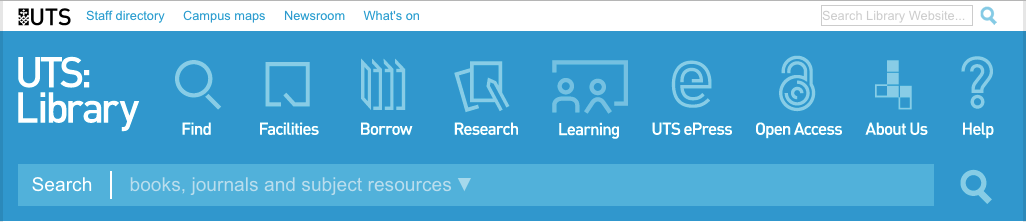
\includegraphics{Images/UTSLibraryBanner.png}

The Library ( \url{http://www.lib.uts.edu.au}) has great resources,
workshops and tools that will help you during your education if you
choose to utilise them.


\includegraphics[width=0.3\linewidth]{Images/HeadsUp}

If you need some help understanding how to use the library, they have
produced some short videos to help you get started:
\url{http://www.lib.uts.edu.au/headsup}


\includegraphics{Images/HeadsUpResearchers_logo_675.png}

The library website has an entire section dedicated to research:
\url{http://www.lib.uts.edu.au/research}

There is also some self paced training modules you can do to help you
get the most of what the library can offer for your research.
\url{http://www.lib.uts.edu.au/headsup-researchers}

\subsection{Searching the catalogue}\label{searching-the-catalogue}

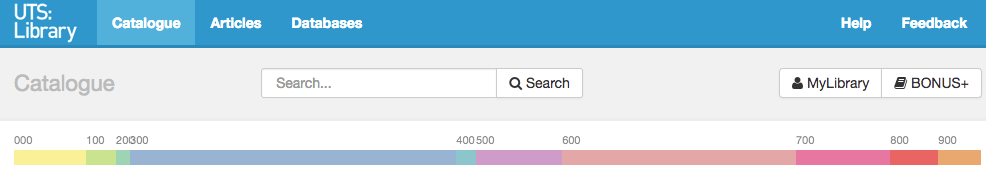
\includegraphics{Images/LibraryCatalogue.png}

One of the great things about the library catalogue is that it returns
results far beyond the resources held by the library itself. UTS pay
subscription fees to many 3rd party resources including journals,
publishers and more. The best thing about this is that if you find
something that has an online source available, you will likely be able
to download a copy to your computer for later reading.

As an example, the link below will take you some search results for the
term ``Data science'' and was then filtered to only show `online'
resources.

\url{http://find.lib.uts.edu.au/search?Ntx=matchallpartial\&Ntk=All\&N=4294967183\&Ntt=data\%20science}

If you click on the `Available' link underneath each resource, it will
then offer you the option of launching the electronic resource.

\subsection{Databases \& Articles}\label{databases-articles}

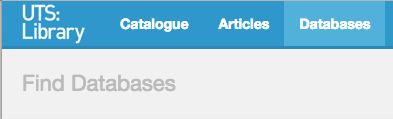
\includegraphics[width=0.4\linewidth]{Images/LibraryDatabases}

If you prefer to search specific sources, you can browse the databases
section for 3rd party providers. This includes sources that UTS
subscriptions that allow you access as a student.

Similarly if you wish to focus your search for specific journal articles
rather than journals or books, the `Articles' button is a great place to
go.

\subsection{Referencing}\label{referencing}

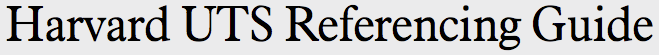
\includegraphics{Images/RefGuide.png}

It is really important that you get used to referencing from the start.
UTS uses the Harvard Referencing style. Fortunately there is an
interactive referencing guide available through the library to make
things easier:

\url{http://www.lib.uts.edu.au/help/referencing}

Make sure to browse through some of the other links at the above link.
You might find some other useful tips (tools).

\subsection{Library events \& tours}\label{library-events-tours}

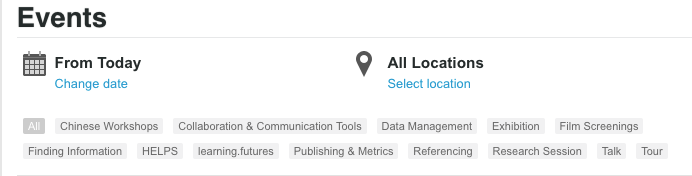
\includegraphics[width=0.5\linewidth]{Images/LibraryEvents}

The library team will help you wherever they can. It is recommended that
you keep an eye out for all their events on
\url{http://www.lib.uts.edu.au/events}

The following events, particularly for MDSI students, are coming up in
the next month and below are links where you can register.

\textbf{MDSI: Data Science Research and Referencing} Tue, 14 March, 2017
\textbf{10:00 AM to 11:30 AM} This workshop is a practical introduction
to advanced research skills and reference management tools, with a focus
on data science. Laptops are recommended but not essential.
Participation is open to MDSI students. A concurrent workshop will run
if more than 24 participants register for this session.
\url{http://www.lib.uts.edu.au/event/609872/mdsi-data-science-research-and-referencing}

\textbf{MDSI: Library Tour and Scavenger Hunt} Tue, 14 March, 2017
\textbf{6:00 PM to 7:00 PM} An interactive tour (it's a scavenger hunt)
of the UTS Library services and facilities for MDSI students. Meet in
the Library foyer.
\url{https://www.lib.uts.edu.au/event/609880/mdsi-library-tour-and-scavenger-hunt}

\section{Professional Experience}\label{professional-experience}

At times Industry will approach CIC for students who might be interested
in internships. These are posted by the CIC:MDSI team in CICAround
whenever these possibilities comes up.

You can find the postings on CICAround
(\url{https://ca.uts.edu.au/blog/})

\section{Data Security}\label{data-security}

include a security/privacy sub section (must cover concepts of masking,
encrypting etc data)

Data security is defined as measures that is used to protect digital
privacy as to prevent unauthorised access to computers, databases,
websites and other digital items. It also protects data from corruption.

Data security can include backups, data masking, encryption or even data
erasure.

Data masking is defined as the process of changing certain part of data
so that the structure remains the same but the information itself is
changed to protect sensitive information. It ensures that sensitive
information is unavailable beyond the permitted environment. It ensures
that the original values are not re-engineered or identified. Eg is user
training and software testing.

Data encryption ensures that data is unreadable to users who are not
authorised to access the data and who do not have the `key'.

One of the most common ways of securing data is using authentication
like passwords, and other data that can verify an identity ( like email
and password login) prior to granting access to a system. These measures
are taken to ensure hackers that use alternative system access methods
to sabotage computer systems and networks.

Hacker actions can be illegal or legal depending on the purpose behind
the actions. There are three categories of hackers :

\begin{itemize}
\tightlist
\item
  Black hat hackers break into computer systems illegally and cause harm
  by stealing or destroying data, i.e., a banking system to steal money
  for personal gain.
\item
  White hat hackers use their skills to help enterprises create robust
  computer systems.
\item
  Grey hat hackers perform illegal hacking activities to show off their
  skills, rather than to achieve personal gain.
\end{itemize}

\textbf{10 General Data Security Tips:}

\begin{enumerate}
\def\labelenumi{\arabic{enumi}.}
\tightlist
\item
  Back up early and often
\item
  Use file-level and share-level security
\item
  Password protect documents
\item
  Use EFS encryption
\item
  Use disk encryption
\item
  Use a public key infrastructure
\item
  Hide data
\item
  Protect data in transit
\item
  Secure wireless transmission
\item
  Use management or access control
\end{enumerate}

\textbf{Types of Encryption:}

\begin{itemize}
\tightlist
\item
  Triple DES : It uses three individual keys with 56 bits each that adds
  up to 168 bits. This is a dependable hardware encryption solution
\item
  RSA : A public-key encryption algorithm and is standard for encrypting
  data over the internet. Is a asymmetric algorithm due to use of a pair
  of keys. There is a public key, to encrypt, and a private key, used to
  decrypt.
\item
  Blowfish : the symmetric cipher splits messages into blocks of 64 bits
  and encrypts them individually. Its high speed and very effective.
  It's also free source software.
\item
  Twofish : Symmetric algorithm with keys up to 256 bits, only one key
  is needed. The fastest of its kind and ideal for hardware and
  software. It's also free source software.
\item
  AES : Most trusted algorithm by U.S. Government. Has an efficient
  128-bit but also a 192 and 256 bit algorithms for heavy duty
  encryption purposes. Considered impervious to attacks except brute
  force.
\item
  Honey Encryption : deters hackers by serving fake data for every
  incorrect guess. It slows down attackers but also provides a haystack
  of false hopes and makes it difficult for hackers to find the correct
  key.
\end{itemize}

\url{http://www.computerworld.com/article/2546352/data-center/top-10-ways-to-secure-your-stored-data.html}

\url{http://www8.hp.com/us/en/software-solutions/what-is/data-security.html}

\url{http://www.lexisnexis.com.au/en-au/products/privacy-confidentiality-and-data-security.page}

\section{Hackathons}\label{hackathons}

Hackathons are competitions (socially or sometimes for a prize) that
challenge you with a goal or a problem. In a data science context this
typically involves datasets and your wits against a clock. Hackathons
are a fantastic way to learn from each other, to ideate, validate,
develop your skills and sometimes even build a prototype. Hackathons are
one of the most authentic learning experiences you can have as a data
science student. You will practice all sorts of skills you need to
become amazing:

\begin{itemize}
\tightlist
\item
  Team work
\item
  How to frame a problem
\item
  Data investigation
\item
  Practicing and learning all kinds of technical skills
\item
  Data storytelling
\item
  Presentation \& selling your ideas
\item
  Networking
\end{itemize}

Hackathons are educational, engaging and empowering. You do not need to
feel ready before you participate. The only thing you need to do is show
up, have a positive `can do' attitude and have fun.

They last anything from a few hours to a few days.

MDSI students have been leaving their mark at these events by taking
home the prizes as well as the really big prize checks as can be seen on
display in CIC.

The most popular one to get involved in is `Unearthed':
\url{http://unearthed.solutions/} Our very own `Data Cake' took home the
first prize in 2016, `Perry's Fan Club' took home shared second prize in
2016 as well as `Team Beaver' taking home Young Innovator Award.

If you don't want to wait for an event and want to sink your teeth into
a hackathon right now, you can participate in online data science
competitions. Here are a few links to get your started:

\begin{itemize}
\tightlist
\item
  Kaggle \url{https://www.kaggle.com/}
\item
  DrivenData \url{https://www.drivendata.org}
\item
  InnoCentive \url{https://www.innocentive.com/ar/challenge/browse}
\end{itemize}

A list of hackathons updated weekly :
\url{http://disruptorshandbook.com/big-list-hackathons/} Another good
source of hackathons : \url{http://www.hackathonsaustralia.com/}

\section{Cloud Computing}\label{cloud-computing}

Cloud computing is a phrase used to describe the act of doing things
that you could do on your own computer but doing it on a remote computer
instead. There several reasons why you might choose to do this. In the
context of data science, this is usually to take advantage of `compute
clusters'.

Compute clusters are exactly what it sounds like. A cluster of computer
processors are used together to give you the advantage of their combined
power which leads to faster data processing. This makes it possible to
run analysis routines on large datasets (gigabytes, terabytes or even
petabytes) that could take days or weeks to run on your laptop, in mere
minutes or hours. There are a few more concepts to understand, but
essentially the bottom line is that cloud computing makes things faster
and big datasets more accessible from an analysis point of view.

There are several providers that operate in this space for data science
purposes. Some of these include:

\begin{itemize}
\tightlist
\item
  Amazon Web Services (AWS)
  \url{https://aws.amazon.com/big-data/?nc2=h_l3_bh}
\item
  Microsoft Azure
  \url{https://azure.microsoft.com/en-us/services/machine-learning/}
\item
  Google Cloud Platform \url{https://cloud.google.com/}
\end{itemize}

Make sure you claim your \$100 student credit when you sign up to the
Github student pack \url{https://education.github.com/pack}

\section{\texorpdfstring{The art of `self
learning'}{The art of self learning}}\label{the-art-of-self-learning}

Self learning is the process of teaching `self'. With the boom in freely
available technology it has become possible for each student to dictate
their own learning experience and how much they want to expand. They can
either learn the minimum of what is being taught in class, or they can
put in extra time and work and participate in the exciting adventure of
self learning.

This involves using various resources from YouTube, Journals, Additional
Books and anything else you can get your hands on that adds to your
skillset and your knowledge base.

In recent days self learning is considered an art with lecturers there
as guidance or mentors on this journey where you can develop your skills
to great depth in a short amount of time.

There are a few things to keep in mind during this journey :

\begin{itemize}
\tightlist
\item
  Reputable sources for learning a concept is required. If you plan to
  embark on the art of self learning you need to make sure that the
  sources you are learning from, know what they are talking about. What
  can be considered reputable sources?

  \begin{itemize}
  \tightlist
  \item
    Academic journals or white papers
  \item
    Non- biased sources
  \item
    Generally, personal blogs are avoided. However, in this constantly
    updating space we might need to learn from other expert in the field
    that explain these fast changing concepts.
  \end{itemize}
\item
  Read textbooks and books about the topic. A large collection of books
  are available to you as a student for free via the Library (you can
  sometimes even download a pdf version for your personal use).
\item
  Watch the videos on YouTube on the topic, especially for the more
  tricky, hands on or mathematical based subjects.
\item
  Learn from your surroundings. Never underestimate the value others can
  bring to your journey. This ranges from mentors to other students,
  some students are further in their journey and can help you along.
  There are also various meet-ups and networking events surrounding
  these topics.
\item
  Hands-on experience is by far the best. Join a hackathon, or get an
  internship.
\item
  Use guided learning experiences, like MOOC's on Coursera or a range of
  other platforms.
\item
  Plan your success. Write down your goals, learning outcomes and what
  you would like to master or be able to do and endeavour to move toward
  those goals (this will be really handy in iLab too).
\end{itemize}

\section{Resources and learning}\label{resources-and-learning}

Online short courses:

\begin{itemize}
\tightlist
\item
  \textbf{Lynda.com} : you have free membership via the Library which
  gives you access to all the courses,
  \url{https://www.lib.uts.edu.au/goto?url=https://shib.lynda.com/Shibboleth.sso/InCommon?providerId=https://aaf-login.uts.edu.au/idp/shibboleth}
\item
  \textbf{Coursera} : membership is free,
  \url{https://www.coursera.org/}
\item
  \textbf{DataCamp} : you have free membership via MDSI which gives you
  access to all the courses, \url{https://www.datacamp.com/}, once you
  join ask to join MDSI group and the courses open up.
\end{itemize}

Online Books:

\begin{itemize}
\tightlist
\item
  \textbf{R for Data Science} by Garrett Grolemund and Hadley Wickham -
  \url{http://r4ds.had.co.nz/}
\item
  \textbf{Applied Predictive Modelling} by Max Kuhn - available via the
  library
  \url{https://link-springer-com.ezproxy.lib.uts.edu.au/book/10.1007\%2F978-1-4614-6849-3}
  (requires login with yoru student ID and password)
\item
  \textbf{Python Data Science} by Jake VanderPlas
  \url{https://github.com/jakevdp/PythonDataScienceHandbook}
\end{itemize}

Github repositories with great links:

\begin{itemize}
\tightlist
\item
  \textbf{Free programming books}
  \url{https://github.com/vhf/free-programming-books/blob/master/free-programming-books.md\#python}
\item
  \textbf{Python Data Science tutorials:}
  \url{https://github.com/ujjwalkarn/DataSciencePython}
\item
  \textbf{R Data Science tutorials:}
  \url{https://github.com/ujjwalkarn/DataScienceR}
\item
  \textbf{Machine learning \& Deep learning tutorials:}
  \url{https://github.com/ujjwalkarn/Machine-Learning-Tutorials/blob/master/README.md}
\item
  \textbf{Some more Github resources and corners of the web to explore:}
  \url{https://www.analyticsvidhya.com/blog/2016/09/most-active-data-scientists-free-books-notebooks-tutorials-on-github/}
\end{itemize}

\chapter{Contributors to FlipAround}\label{contributors-to-fliparound}

\begin{tabular}{l|l}
\hline
What & Who.did.it.for.you\\
\hline
FlipAround Team & Zherish Opperman; Detlev Kerkovius; Rory Angus; Dorotea Baljevic; Herry Basuki\\
\hline
Editorial & Zherish Opperman; Detlev Kerkovius\\
\hline
Content & Zherish Opperman; Detlev Kerkovius; Amela Peric; Theresa Anderson\\
\hline
Layout & Zherish Opperman; Detlev Kerkovius; Amela Peric; Theresa Anderson\\
\hline
\end{tabular}


\end{document}
